%==============================================================================
% Sjabloon poster bachproef
%==============================================================================
% Gebaseerd op document class `a0poster' door Gerlinde Kettl en Matthias Weiser
% Aangepast voor gebruik aan HOGENT door Jens Buysse en Bert Van Vreckem

\documentclass[a0,portrait]{hogent-poster}

% Info over de opleiding
\course{Bachelorproef}
\studyprogramme{toegepaste informatica}
\academicyear{2023-2024}
\institution{Hogeschool Gent, Valentin Vaerwyckweg 1, 9000 Gent}

% Info over de bachelorproef
\title{De beste JavaScript runtime-omgeving voor performante applicaties: een vergelijkende studie}
% \subtitle{Ondertitel (eventueel)}
\author{Quinten De Wolf}
\email{quinten.dewolf2@student.hogent.be}
\supervisor{Martine Van Audenrode}
\cosupervisor{Dmitriy Van Der Elst (Cognit bv. - Involv Intranet)}

% Indien ingevuld, wordt deze informatie toegevoegd aan het einde van de
% abstract. Zet in commentaar als je dit niet wilt.
\specialisation{Mobile en Enterprise development}
\keywords{Bun, Node.js, backend}
\projectrepo{https://github.com/user/repo}

\begin{document}

\maketitle

\begin{abstract}
In de voorbije jaren zijn er voortdurend nieuwe javascript runtime-omgevingen ontwikkeld met telkens nieuwe verbeteringen. 
Echter worden weinig van deze nieuwe ontwikkelingen effectief in de praktijk gebruikt.
Zo is het oudere Node.js nog altijd de standaard in de industrie. 
In dit onderzoek wordt bestudeerd of deze nieuwere frameworks een meerwaarde bieden op vlak van performantie.
De onderzoeksvraag hierbij is of één van deze nieuwe frameworks  
een correcte plaatsvervanger kan zijn voor Node.js bij de ontwikkeling van webapplicaties binnen bedrijven 
waar performantie centraal staat.
Hiervoor werd voor beide frameworks een proof-of-concept gemaakt waarop performantie testen werden uitgevoerd.
Doormiddel van de testresultaten kon de performantie tussen de twee frameworks worden vergeleken.
Daarnaast werden ook een vergelijking tussen hun respectievelijke package managers uitgewerkt. 
Het resultaat zijn verschillende metingen van beide frameworks die kunnen worden vergeleken.
Er wordt hierbij verwacht dat het nieuwe framework Bun beter presteert dan Node.js door zijn focus op performantie.
Op basis van deze vergelijking kan een onderbouwde keuze worden gemaakt bij de selectie van een javascript runtime-omgeving.
\end{abstract}

\begin{multicols}{2} % This is how many columns your poster will be broken into, a portrait poster is generally split into 2 columns

\section{Introductie}
Node.js is nog altijd de standaard keuze bij JavaScript runtime-omgevingen. 
Echter zijn er tal van andere omgevingen die de specifieke noden vervullen waar Node.js niet kan aan voldoen.
Zo is de nood voor een goede performantie doorheen de tijd alsmaar belangrijker geworden bij JavaScript backend applicaties.
Bun probeert hierop in te spelen door een performantere omgeving aan te bieden. 
In dit onderzoek wordt dieper ingegaan op deze performantie en wordt deze vergeleken met de performantie van Node.js.
Op basis van de resultaten kan een weloverwogen keuze gemaakt worden bij de ontwikkeling van JavaScript backend applicaties.
Specifiek worden aan de hand van de metingen bij de proof-of-concepts volgende vragen beantwoord:
\begin{itemize}
  \item Wat zijn de onderliggende verschillen tussen Node.js en Bun?
  \item Is de Bun performanter dan Node.js bij het uitvoeren van computationele berekeningen?
  \item Is de Bun performanter dan Node.js bij het afhandelen van netwerkverzoeken?
  \item Wat is het verschil tussen hun respectievelijke package managers?
\end{itemize}
\section{Methodologie}
Het onderzoek bevat 4 fasen. 
In de eerste fase wordt een beter begrip over de JavaScript runtime-omgevingen en het onderzoeksdomein bekomen aan de hand van een literatuurstudie.
In de tweede fase wordt, aan de hand van een requirementsanalyse, één omgeving geselecteerd om performantie te vergelijken met Node.js.
In de derde fase worden de zelfgemaakte proof-of-concepts opgesteld en getest voor beide omgevingen. 
Hierbij wordt een applicatie ontwikkeld waarbij een gebruiker onderwerpen kan ophalen en beoordelen, alsook een script dat het QuickSort algoritme uitvoert.
Aan de hand van de resultaten komen we tot de laatste namelijk de conclusie. Hierbij wordt de data geïnterpreteerd om een antwoord te formuleren op de onderzoeksvragen.
Uit deze antwoorden kan afgeleid worden of Bun een geschikte plaatsvervangen kan zijn voor Node.js binnen de ontwikkeling van performantie backend applicaties.
\begin{center}
  \captionsetup{type=figure}
  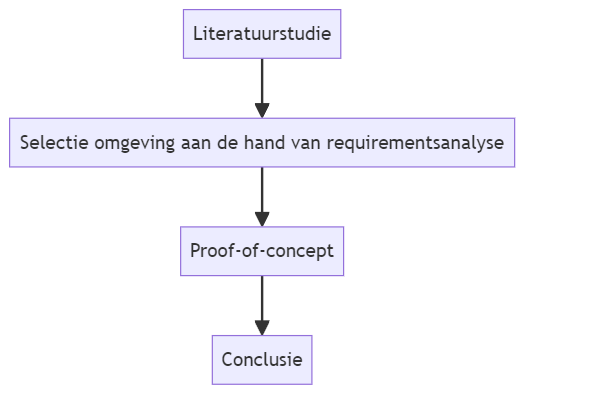
\includegraphics[width=1.0\linewidth]{flowchart}
  \captionof{figure}{Flowchart van de methodologie}
\end{center}


\section{Experimenten}

De metingen worden uitgevoerd met behulp van 2 benchmark tools, Hyperfine en Bombardier, om volgende zaken te kunnen meten:
\begin{itemize}
    \item De latentie van de applicatie.
    \item Het aantal verzoeken per seconde bij de applicatie.
    \item De uitvoeringstijd van de berekeningen van het QuickSort algoritme.
    \item Het geheugengebruik bij de applicatie.
    \item De installatietijd voor de respectievelijke package managers.
    \item Het CPU-gebruik bij de applicatie.
\end{itemize}
Bij de applicatie worden de metingen zowel bij een MySQL databank als bij een PostgreSQL databank uitgevoerd met behulp van een ORM.
\begin{center}
  \captionsetup{type=figure}
  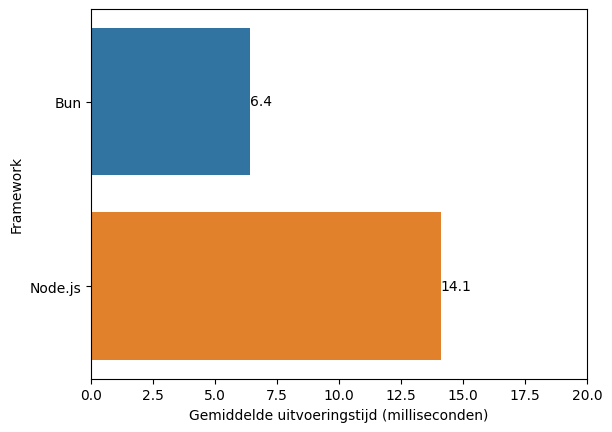
\includegraphics[width=1.0\linewidth]{scriptuitvoeringstijd}
  \captionof{figure}{Uitvoeringstijd van het QuickSort algoritme}
\end{center}
Bij het QuickSort algoritme had Bun een snellere uitvoeringstijd dan Node.js, wat aantoont dat Bun computationeel sneller is dan Node.js.


\section{Conclusies}

Don't underestimate the Force. Oh God, my uncle. How am I ever gonna explain this? I suggest you try it again, Luke. This time, let go your conscious self and act on instinct. Don't be too proud of this technological terror you've constructed. The ability to destroy a planet is insignificant next to the power of the Force.

\section{Toekomstig onderzoek}

I care. So, what do you think of her, Han? No! Alderaan is peaceful. We have no weapons. You can't possibly… I have traced the Rebel spies to her. Now she is my only link to finding their secret base.

Kid, I've flown from one side of this galaxy to the other. I've seen a lot of strange stuff, but I've never seen anything to make me believe there's one all-powerful Force controlling everything. There's no mystical energy field that controls my destiny. It's all a lot of simple tricks and nonsense. You are a part of the Rebel Alliance and a traitor! Take her away! 

\end{multicols}
\end{document}